%% SC4064 Assignment 3 — Performance Analysis Report
\documentclass[
hf,
]{confart}

\sloppy

\usepackage{listings}
\usepackage{booktabs}
\usepackage{tabularx}
\usepackage{xcolor}
\usepackage{amsmath}
\usepackage{graphicx}

\definecolor{codegreen}{rgb}{0,0.6,0}
\definecolor{codegray}{rgb}{0.5,0.5,0.5}
\definecolor{codepurple}{rgb}{0.58,0,0.82}
\definecolor{backcolour}{rgb}{0.95,0.95,0.92}
\lstdefinestyle{mystyle}{
    backgroundcolor=\color{backcolour},
    commentstyle=\color{codegreen},
    keywordstyle=\color{magenta},
    numberstyle=\tiny\color{codegray},
    stringstyle=\color{codepurple},
    basicstyle=\ttfamily\footnotesize,
    breakatwhitespace=false,
    breaklines=true,
    captionpos=b,
    keepspaces=true,
    numbers=left,
    numbersep=5pt,
    showspaces=false,
    showstringspaces=false,
    showtabs=false,
    tabsize=2
}
\lstset{style=mystyle, breaklines=true}

\begin{document}

\setConferenceHeader{SC4064 GPU Programming — Assignment 3}
\copyrightyear{2026}
\copyrightclause{}
\conference{SC4064 GPU Programming, NTU, 2026.}

\title{GPU-Accelerated Image Processing Pipeline: Performance Analysis}

\author[1]{Qian Jianheng Oscar}[%
email=qian0081@e.ntu.edu.sg,
]

\address[1]{Nanyang Technological University, Singapore}

\ExplSyntaxOn
\cs_if_free:cTF { g_conf_logonote_seq } { \seq_new:N \g_conf_logonote_seq } { }
\ExplSyntaxOff

\maketitle

%% ════════════════════════════════════════════════════════════════════
\section{Roofline Analysis}
\label{sec:roofline}

All measurements were taken on an NVIDIA H100 80GB HBM3 (SXM variant, compute capability 9.0) with peak FP32 throughput of 67~TFLOP/s (CUDA cores) and peak memory bandwidth of 3.35~TB/s. The ridge point is at $67 / 3.35 \approx 20.0$~FLOPs/byte. Images are $512 \times 512$ greyscale (262\,144~pixels).

\subsection{Arithmetic Intensity}

\paragraph{Gaussian Blur.}
Each output pixel requires a 5$\times$5 convolution: 25 multiplications and 24 additions (summing 25 weighted values) = \textbf{49~FLOPs} per pixel. With shared-memory tiling, global memory traffic is reduced to reading the input image once and writing the output once: \textbf{2~bytes/pixel}. This gives an arithmetic intensity of $49 / 2 = \mathbf{24.5}$~FLOPs/byte. In a na\"ive (no tiling) implementation, each pixel is read up to 25 times by neighbouring output threads, yielding 26~bytes/pixel and AI $= 49/26 = 1.88$~FLOPs/byte.

\paragraph{Sobel Edge Detection.}
The Sobel kernel reads a 3$\times$3 neighbourhood and computes two convolutions ($G_x$, $G_y$) using integer arithmetic (not counted as FLOPs). The only floating-point operations are: $G_x^2$ (1~mul), $G_y^2$ (1~mul), $G_x^2 + G_y^2$ (1~add), and $\sqrt{\cdot}$ (1~FLOP) = \textbf{4~FLOPs} per pixel. Without shared-memory tiling, each pixel is read up to 9 times from global memory, giving 10~bytes/pixel (9~reads + 1~write) and AI $= 4/10 = \mathbf{0.40}$~FLOPs/byte.

\paragraph{Histogram + Equalisation.}
The histogram kernel performs zero floating-point operations (only integer \texttt{atomicAdd}). The equalisation kernel performs 4~FLOPs per pixel: 1~subtraction ($\text{CDF}[v] - \text{CDF}_{\min}$), 1~subtraction ($W \times H - \text{CDF}_{\min}$), 1~division, and 1~multiplication ($\times 255$). Combined global memory traffic is $\sim$3~bytes/pixel (1~byte read for histogram + 1~byte read + 1~byte write for equalisation). Combined AI $= 4/3 = \mathbf{1.33}$~FLOPs/byte.

\begin{table}[htbp]
\centering
\renewcommand{\arraystretch}{1.1}
\begin{tabularx}{\columnwidth}{l*{4}{>{\centering\arraybackslash}X}}
\toprule
\textbf{Kernel} & \textbf{FLOPs/px} & \textbf{Bytes/px} & \textbf{AI (F/B)} & \textbf{Time (ms)} \\
\midrule
Gaussian Blur (tiled) & 49 & 2 & 24.50 & 0.0088 \\
Gaussian Blur (na\"ive) & 49 & 26 & 1.88 & --- \\
Sobel & 4 & 10 & 0.40 & 0.0073 \\
Histogram + Equalise & 4 & 3 & 1.33 & 0.095\textsuperscript{*} \\
\bottomrule
\end{tabularx}
\caption{Arithmetic intensity and measured kernel times. \textsuperscript{*}Includes histogram (0.065~ms), thrust CDF (0.024~ms), and equalise (0.007~ms).}
\label{tab:ai}
\end{table}

\subsection{Roofline Plot}

Figure~\ref{fig:roofline} plots each kernel on the H100 roofline. The ridge point at 20.0~FLOPs/byte separates the memory-bound (left) and compute-bound (right) regions.

\begin{figure}[htbp]
    \centering
    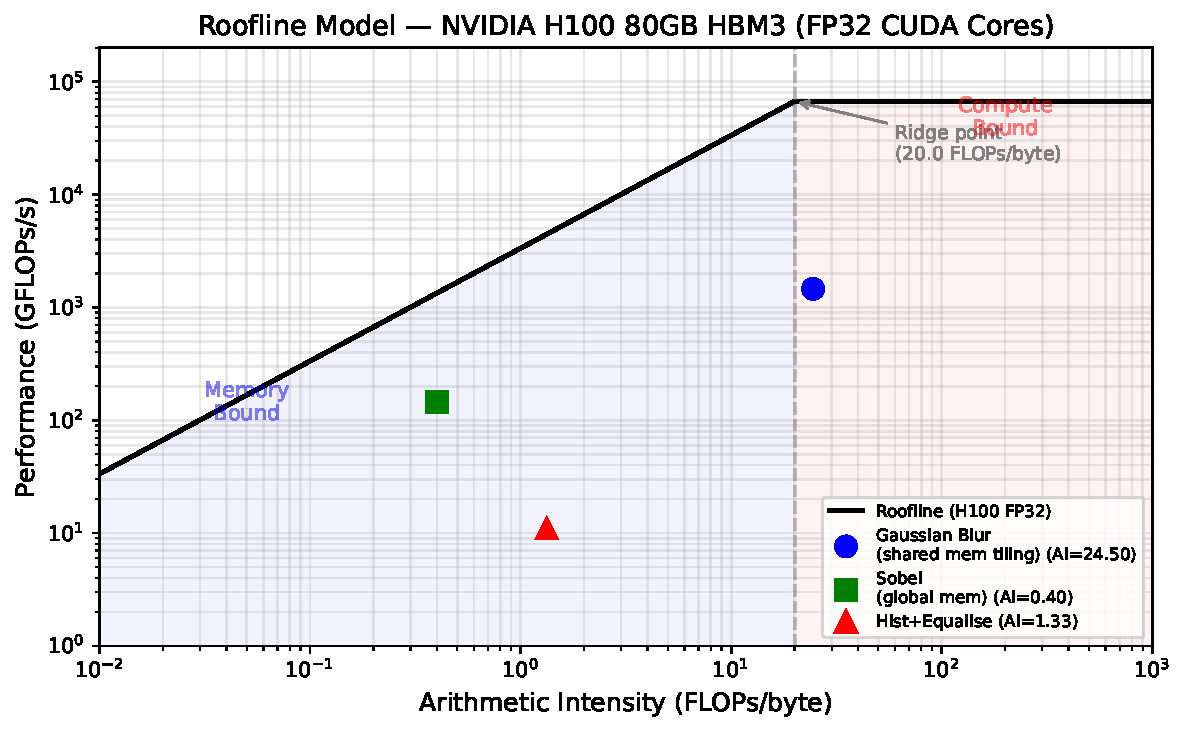
\includegraphics[width=0.95\columnwidth]{assets/roofline.pdf}
    \caption{Roofline plot for NVIDIA H100 80GB HBM3 (FP32 CUDA cores). Each kernel is plotted at its (AI, achieved GFLOPs/s).}
    \label{fig:roofline}
\end{figure}

\subsection{Interpretation}

\paragraph{Gaussian Blur} sits near the ridge point (AI = 24.5) and achieves 1,461~GFLOPs/s — about 2.2\% of peak FP32 compute. The kernel is close to the memory-bound/compute-bound transition. Shared-memory tiling reduced global memory traffic by $13\times$ compared to na\"ive (from 26 to 2 bytes/pixel), which shifts the kernel from clearly memory-bound (AI = 1.88) to near the ridge. The achieved bandwidth (tiled) is only $\sim$60~GB/s, far below peak (3.35~TB/s), suggesting the kernel is limited by the small image size (512$\times$512 = 262K pixels) which does not generate enough threads to saturate the H100's large number of SMs.

\paragraph{Sobel} is deeply memory-bound (AI = 0.40, well left of the ridge). Its achieved bandwidth is $\sim$361~GB/s ($\sim$10.8\% of peak). The low AI means performance is entirely limited by memory throughput. Adding shared-memory tiling would reduce bytes/pixel from 10 to 2, increasing AI to 2.0, but the kernel would remain memory-bound.

\paragraph{Histogram + Equalise} is memory-bound (AI = 1.33). The histogram kernel is the pipeline bottleneck at 0.065~ms — over 7$\times$ slower than the blur kernel — due to contention on atomic operations to the 256 global histogram bins. A per-block shared-memory histogram would reduce this contention.

\paragraph{Pipeline Bottleneck.}
The histogram kernel dominates at 59\% of total kernel time. To improve overall throughput: (1) use per-block shared-memory histogram to reduce atomic contention; (2) process larger images or larger batches to better utilise the H100's massive parallelism; (3) fuse the equalise kernel with a subsequent pipeline stage to reduce memory round-trips.

%% ════════════════════════════════════════════════════════════════════
\section{Stream Overlap Analysis}
\label{sec:streams}

Our pipeline creates one CUDA stream per image and enqueues all operations (H$\to$D transfer, blur, Sobel, histogram, equalise, D$\to$H transfer) on that stream. Operations within a single stream execute in order, while operations on different streams can overlap.

\paragraph{Overlap limitation.}
In the current implementation, \emph{no meaningful overlap} occurs between streams. The root cause is \texttt{thrust::exclusive\_scan}, which executes on the default (NULL) stream. Before calling thrust, we must call \texttt{cudaStreamSynchronize(streams[i])} to ensure the histogram kernel has completed. Thrust then runs on the default stream, which implicitly synchronises with all other streams, serialising the entire pipeline per image.

This means that while image $i$ is computing its CDF via thrust, no other image's kernels can execute. The pipeline effectively degenerates to sequential per-image processing.

\paragraph{Is it a pinned memory issue?}
No. Host buffers are allocated with \texttt{cudaMallocHost} (pinned memory), which correctly enables asynchronous DMA transfers. The H$\to$D and D$\to$H \texttt{cudaMemcpyAsync} calls are genuinely asynchronous.

\paragraph{Is it a hardware constraint?}
No. The H100 has a copy engine that can overlap with compute. The issue is purely in the stream design.

\paragraph{Fix.}
To achieve overlap, the CDF computation should avoid the default stream. Options include: (1) implement a custom prefix-scan kernel launched on the per-image stream; (2) use thrust's execution policy with per-stream dispatch (\texttt{thrust::cuda::par.on(streams[i])}); or (3) compute the CDF entirely on the host after a single device$\to$host copy of the 256-entry histogram, avoiding any GPU-side scan.

%% ════════════════════════════════════════════════════════════════════
\section{Multi-GPU Speedup Analysis}
\label{sec:multigpu}

\begin{table}[htbp]
\centering
\renewcommand{\arraystretch}{1.1}
\begin{tabular}{lcc}
\toprule
\textbf{Configuration} & \textbf{Time (ms)} & \textbf{Speedup} \\
\midrule
1 GPU (20 images)  & 25.26 & 1.00$\times$ \\
2 GPUs, sequential & 25.32 & 1.00$\times$ \\
\bottomrule
\end{tabular}
\caption{End-to-end GPU processing time (excluding file I/O), averaged over 200 runs with pre-allocated buffers.}
\label{tab:multigpu}
\end{table}

\paragraph{Achieved speedup.}
The measured speedup with two GPUs is effectively \textbf{1.00$\times$} (no improvement). This is because the current implementation calls \texttt{process\_batch\_on\_device} \emph{sequentially}: GPU~0 processes its 10 images, then GPU~1 processes its 10 images. The two GPUs never run concurrently.

\paragraph{Why not 2$\times$?}
Even with concurrent GPU execution (e.g., using \texttt{std::thread}), the \texttt{thrust::exclusive\_scan} serialisation discussed in Section~\ref{sec:streams} would limit overlap. Additionally, 512$\times$512 images are small — each image's kernels complete in $<$0.1~ms, so the pipeline is dominated by CPU-side overhead (thrust calls, CDF host copies, stream synchronisation) rather than GPU compute.

\paragraph{Amdahl's Law for 4 GPUs.}
Let $f$ be the fraction of work that is parallelisable across GPUs. The serial fraction includes: thrust CDF computation (runs on default stream, blocking), host-side CDF minimum search, and stream synchronisation overhead. From our measurements, kernel time is $\sim$2.2~ms for 20 images while total time is 25.3~ms, giving a serial fraction of approximately $s = (25.3 - 2.2)/25.3 \approx 0.91$. Amdahl's Law predicts:

\[
S(n) = \frac{1}{s + (1-s)/n} = \frac{1}{0.91 + 0.09/4} \approx 1.07\times
\]

Even with 4 GPUs, the predicted speedup is only $\sim$1.07$\times$, because 91\% of the runtime is serial overhead.

\paragraph{Practical factors beyond Amdahl's Law.}
(1)~\textbf{PCIe contention}: multiple GPUs share PCIe bandwidth for H$\to$D/D$\to$H transfers, reducing effective bandwidth per GPU. (2)~\textbf{NUMA effects}: pinned host memory may be allocated on one NUMA node, causing remote access latency for GPUs attached to a different node. (3)~\textbf{CPU scheduling}: with $n$ GPUs, the host must manage $n$ times more streams and thrust calls, increasing CPU-side serialisation. (4)~\textbf{Device switching overhead}: \texttt{cudaSetDevice} incurs a context switch cost that grows with the number of GPUs.

\end{document}
